\documentclass[12pt]{article}

\usepackage{sbc-template}

\usepackage{graphicx,url}

%\usepackage[brazil]{babel}   
\usepackage[latin1]{inputenc}  

     
\sloppy

\title{Instructions for Authors of SBC Conferences\\ Papers and Abstracts}

\author{Tiago O. de Farias\inst{1}}


\address{UniRitter Laureate International Universities\\
  Rua Orfanatr�fio, 555 - Alto Teres�polis - 90840-440 - Porto Alegre - RS - Brasil
  \email{tiago.farias.poa@gmail.com}
}

\begin{document} 

\maketitle

\begin{abstract}
  
\end{abstract}
     
\begin{resumo} 
  
\end{resumo}


\section{Introdu��o}



\section{Referencial Te�rico} \label{sec:firstpage}



\section{Estado da Arte}



\section{Solu��o Implementada}



\subsection{Subsections}

The subsection titles must be in boldface, 12pt, flush left.

\section{Considera��es Finais}

\section{Figures and Captions}\label{sec:figs}


Figure and table captions should be centered if less than one line
(Figure~\ref{fig:exampleFig1}), otherwise justified and indented by 0.8cm on
both margins, as shown in Figure~\ref{fig:exampleFig2}. The caption font must
be Helvetica, 10 point, boldface, with 6 points of space before and after each
caption.

\begin{figure}[ht]
\centering
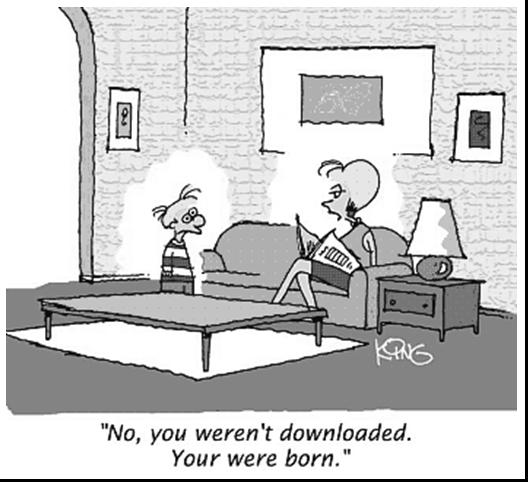
\includegraphics[width=.5\textwidth]{fig1.jpg}
\caption{A typical figure}
\label{fig:exampleFig1}
\end{figure}

\begin{figure}[ht]
\centering
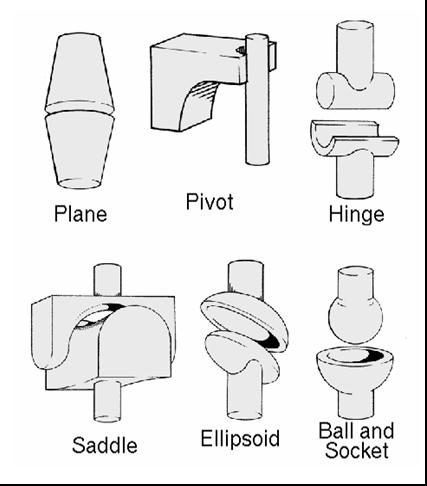
\includegraphics[width=.3\textwidth]{fig2.jpg}
\caption{This figure is an example of a figure caption taking more than one
  line and justified considering margins mentioned in Section~\ref{sec:figs}.}
\label{fig:exampleFig2}
\end{figure}

In tables, try to avoid the use of colored or shaded backgrounds, and avoid
thick, doubled, or unnecessary framing lines. When reporting empirical data,
do not use more decimal digits than warranted by their precision and
reproducibility. Table caption must be placed before the table (see Table 1)
and the font used must also be Helvetica, 10 point, boldface, with 6 points of
space before and after each caption.

\begin{table}[ht]
\centering
\caption{Variables to be considered on the evaluation of interaction
  techniques}
\label{tab:exTable1}
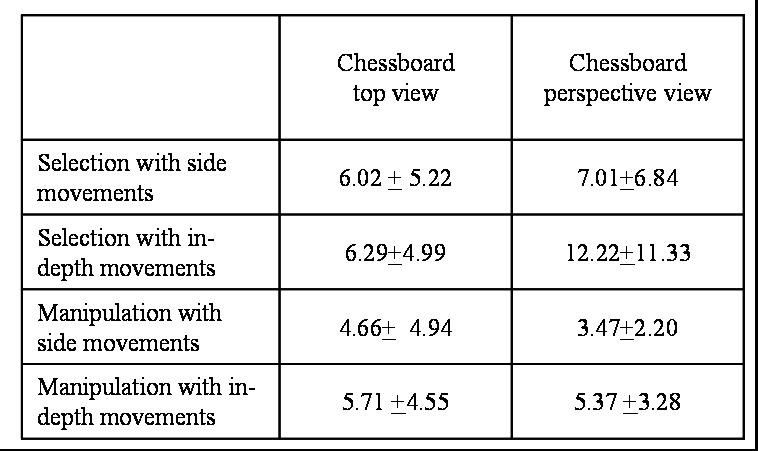
\includegraphics[width=.7\textwidth]{table.jpg}
\end{table}

\section{Referencias}

Bibliographic references must be unambiguous and uniform.  We recommend giving
the author names references in brackets, e.g. \cite{knuth:84},
\cite{boulic:91}, and \cite{smith:99}.

The references must be listed using 12 point font size, with 6 points of space
before each reference. The first line of each reference should not be
indented, while the subsequent should be indented by 0.5 cm.

\bibliographystyle{sbc}
\bibliography{sbc-template}

\end{document}
